
\section{Extending \app and Applying it to Real-World Configurations}
\label{sec:travis}

TravisCI~\cite{API} is a popular integration and build testing service 
connected to Github. It has been used on more than 17 
millions of projects. 
TravisCI allows programmers to automatically run their test suite on a fresh virtual machine every time they commit their code.
A TravisCI user must add a configuration file to the repository that specifies build conditions, 
such as which dependencies are required, and a set of benchmarks to test. 
The results of these tests (indicating either passing, failing, or misconfiguration) 
are saved by TravisCI on a publicly available database~\cite{API}.

TravisCI misconfigurations are important to detect and correct before execution,
because any failed compilation can costs developer significant amount 
of time. A misconfiguration can cause a test suite to run up to 20 
minutes, only to report that the whole computation failed~\cite{API}.
If developer would have this information prior to the compilation attempt, they could
 identifying and correct potential misconfigurations.

A new challenge here is that we need to reason about a 
temporal component too. Having an entire TravisCI log for a given
project we can examine the sequence of changes of a configuration file
and we can detect what has changed so that we switched from a failing 
compilation to successful compilation. 

%Driven by the above motivating example, we propose an extension to \app that
%learns over a training set with both correct and incorrect examples, as well as a temporal structure.
%Such an extension employs an existing technique from the machine learning community, called version space learning,
%to significantly decrease the false positive rate while maintaining the detection capability of \app.

\subsection{Version Space Learning with Temporal Properties} 

We plan to use version space learning and SMT solvers to detect errors in 
TravisCI configurations files. Version space learning 
builds a logical constraint model for binary
classification~\cite{mitchell77}, which we use to test a configuration file for 
membership in the set of all correct files.

\begin{wrapfigure}{l}{0.5\textwidth}
  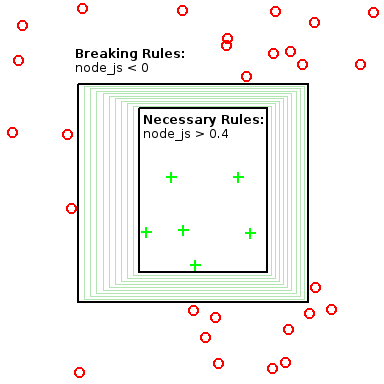
\includegraphics[width=0.45\textwidth]{figs/Version_space}
  \caption{\small Red circles are failing files, and green pluses are passing files.}
  \label{fig:versionSL}
\end{wrapfigure}

Figure~\ref{fig:versionSL} outlines our proposed approach. We first apply the standard ConfigC approach to learn the rules that have 
to hold for correct TravisCI configuration files. Traditionally, 
version space learning builds a model that defines membership using a series of 
disjunctions from a set of predefined hypotheses.  However, we need  to 
use conjunctions to convey that a configuration file is only correct if 
it satisfies all the learned relations. Those rules can be seen as
positive examples in classifying correct files. In addition, we will have
so-called {\emph {breaking rules}} which are derived from the files 
that do not compile, \ie~negative examples. Breaking rules are specified 
using disjunctions.

Figure~\ref{fig:versionSL} shows an example set of necessary and breaking rules that would be learned if the training set contains a failing file indicating that 
{\small node\_js} version is 0.2, and a passing file has its version set to 0.4.
With red dots we depict incorrect files that do not compile, and the green crosses show correct files.
From both types of files, we extract breaking and necessary rules, which define borders between those two sets of files.
This results in a space (green stripes) where a file may contain relations that cannot be classified as either breaking or necessary.
For example, if a user provides a file which specifies version 0.3 of {\small node\_js}, this file will fall in the green striped space.
Part of the research task will be to find an optimal classification for such cases.

The success or failure of a TravisCI configuration file is dependent
not only on the configuration file itself (namely, a .travis.yml file) but it also depends on system information such as programming languages and a list of imported libraries.
For this reason, we call this extended configuration files a program summary, denoted with $P_t$. This is a representation 
of the repository which contains any information 
relevant to the learning process.
The subscript on $P_t$ is a timestamp tag based on 
the ordered git commit history.
%In the case of TravisCI, this include the \verb|.travis.yml| file, 
%as well as code features that may effect build status, 
%such as programming language and a list of imported libraries.
%The summary must be \textit{sufficiently detailed}, that is it must contain every piece of information that might lead to a build error.

%IMPORTANT, but no space
%However, a git history is not a limited to a single linear timeline.
%Git features the ability to \textit{branch}, which allows to simultaneous commit chains.
%To handle the start of a branch, add a superscript to indicate the branch, and restart the counter on a branch.
%To handle the merge of two branches $P_{t}^{x}$ and $P_{t'}^{y}$, step to $P_{t+1}^{x}$, where $x$ is the mainline branch.
%We then say that $P_{t'}^{y}$ has no successor commit $P_{t'+1}^{y}$.

From these summaries we will build a model $M(P_t)$, using the same techniques as in 
\app. $M(P_t)$ actually is a set of all possible relations derivable 
from the program summary. As previously, we need to construct templates for the 
learning process, since the level of specification details depends on them.

We now outline how we plan to use SMT solvers to find the sets of necessary rules ($Nec$), and the set of breaking rules ($Br$).

Let $S(P_t)$ be the build status returned from TravisCI when run on $P_t$.
It can be either $Pass$ or $Err$. We define shorthand $S(P_{t,t+1}) = PE$ (also called a break state), to 
express that the program was compiling before and now it does not:
\begin{align*}
  S(P_{t,t+1}) = PE :\Leftrightarrow S(P_t)=Pass \land S(P_{t+1})=Err 
\end{align*}


If executing a TravisCI file fails, then there must exist at least one rule that is
causing that error. Similarly, if a build is passing, then there must not exist any error.
That is, the model of a passing commit must not contain any breaking rules.
Note we are not, however, guaranteed that any rules from a passing commit are necessary.
\begin{align}
  S(P_t) = Err \Rightarrow \exists r \in  M (P_t), r \in Br \label{eq:E}\\
  S(P_t) = Pass \Rightarrow \forall r \in  M (P_t), r \notin Br \label{eq:P}
\end{align}

%While Eq. \ref{eq:E} and \ref{eq:P} might build a basic model, they will do not capture all of the available knowledge.
%The key insight is that 
Additionally, when we commit a break ($PE$), we can localize the error to one of the relations that changed.
Either we removed something that was necessary, or added something that was breaking.
Note that this is an inclusive disjunction, since a erroring commit can break multiple things at once.
Expressed formally, where $\setminus$ is the set difference, that is:
\begin{align}
  S(P_{t,t+1}) &= PE \Rightarrow \nonumber \\
  \exists& r \in (M(P_{t})\ \setminus M(P_{t+1})), r \in Nec\ \nonumber \\
  \lor \ \exists& r \in (M(P_{t+1}) \setminus M(P_{t})), r \in Br \label{eq:PE}
\end{align}

We then create a conjunction of \eqref{eq:E}, \eqref{eq:P}, and  \eqref{eq:PE} with
conjunctions and invoke an SMT solver to find a model for that formula.
The resulting model will define sets of necessary rules ($Nec$), and the set of breaking rules ($Br$), which can be used to check new configuration files.
Since we used a similar model to \app, we will still be able to provide justifications for the classification results.

We also believe that this approach will work in practice since travis.yml files are relatively small and changes in the files are often at most 1-2 lines.

